\chapter{کار با ترمینال}
از زیرمجموعه‌های لینوکس، رابط‌های گرافیکی یا \lr{GUI}ها هستند (\lr{Graphical User Interface}) که شما در آن می‌توانید موس‌تان را تکان دهید، کلیک کنید و بکشید، و می‌توانید بدون این‌که مستندات زیادی را بخوانید، کارهای‌تان را انجام دهید. محیط سنتی \lr{Unix}، یک رابط خط فرمان یا \lr{CLI} است (\lr{Command Line Interface}) که دستورات را در آن تایپ می‌کنید تا به کامپیوتر بگویید که چه کاری انجام دهد. این روش، خیلی سریع‌تر و قدرتمندتر است؛ اما لازم است که دستورات را بشناسید. در برخی شرایط، مخصوصا هنگام پیکربندی سیستم، مجبوریم که از ترمینال استفاده کنیم.

\section{آشنایی اولیه با ترمینال}
برای بازکردن ترمینال در اوبونتو، کافی است که روی لانچر کلیک کنید و چند حرف از کلمهٔ \lr{Terminal} را تایپ کنید تا آیکون ترمینال ظاهر شود. روی آن کلیک کنید. پنجرهٔ ترمینال باز خواهد شد.\\
در پنجرهٔ بازشده، یک خط مثل \lr{\texttt{ahmad@ahmad-netbook:$\sim$\$}} را مشاهده می‌کنید. \lr{\texttt{ahmad}} نام کاربری کنونی‌تان، \lr{\texttt{ahmad-netbook}} نام رایانهٔ‌تان، \lr{\texttt{$\sim$}} محل پوشهٔ کنونی‌تان (که این علامت، به معنی پوشهٔ خانگی‌تان است) و \lr{\texttt{\$}} هم به معنی دارابودن مجوز عادی و نداشتن مجوز کاربر ریشه است.
\begin{center}
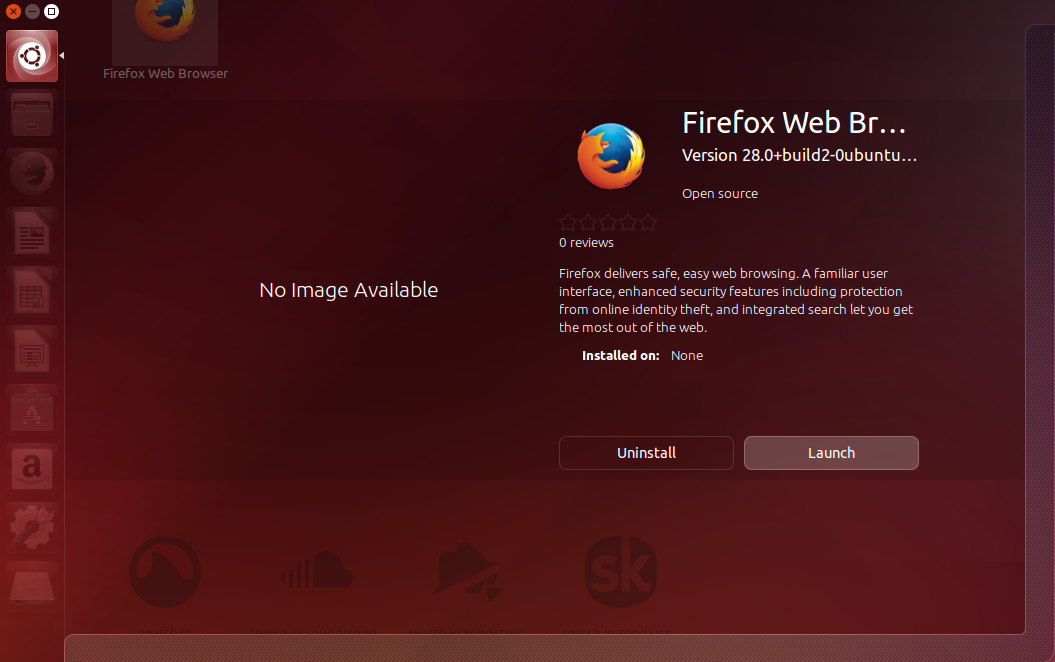
\includegraphics[scale=0.45]{pics/25.png}
\end{center}

\section[،sudo اجرای دستورات با بالاترین مجوز دسترسی]{\lr{sudo}، اجرای دستورات با بالاترین مجوز دسترسی}
بعضی از دستورات، به اضافه‌کردن دستور \lr{\texttt{sudo}} (\lr{Super User Do}) به اولشان نیاز دارند. این در صورتی است که با فایل‌ها و پوشه‌هایی کار کنید که متعلق به حساب کاربری شما نباشد. این یک دستور ویژه است که به صورت موقت، به شما اجازهٔ تغییر تنظیمات کامپیوتر را می‌دهد. پس از واردکردن این دستور، ترمینال از شما گذرواژه را خواهد پرسید. می‌بینید که با واردکردن گذرواژه، چیزی در ترمینال نشان داده نمی‌شود. این کار، برای امنیت بیش‌تر است.

\subsection[تفاوت sudo با su]{تفاوت \lr{sudo} با \lr{su}}
در بسیاری از گنو/لینوکس‌های دیگر، امکان استفاده از دستور \lr{\texttt{sudo}} به صورت پیش‌فرض وجود ندارد. در این توزیع‌ها، به جای \lr{\texttt{sudo}}، از \lr{\texttt{su}} استفاده می‌شود.\\
\lr{\texttt{su}} مخفف عبارت \lr{Substitute User} به معنای «تغییر کاربر» است. یعنی علاوه بر تغییر کاربر کنونی به کاربر ریشه (کاربر ریشه یا \lr{root}، دارای بالاترین مجوز در سیستم‌های یونیکسی است)، می‌توان با واردکردن دستور \lr{\texttt{su \emph{user}}} (که به جای \lr{\texttt{\emph{user}}}، باید نام کاربر مورد نظر را بنویسید)، به عنوان آن کاربر فعالیت کرد. دستور \lr{\texttt{su}} هم وارد حساب کاربری ریشه خواهد شد. با زدن این دستور، خط ترمینال شبیه \lr{\texttt{root@ahmad-netbook:/home/ahmad\#}} خواهد شد. علامت \lr{\texttt{\#}} نشان‌دهندهٔ حضور در حساب کاربری ریشه است.\\
در اوبونتو، امکان استفاده از \lr{\texttt{su}} هم وجود دارد. می‌توان با دستور \lr{\texttt{sudo su}}، وارد حساب کاربری ریشه شد. برای فعال‌کردن \lr{\texttt{su}}، باید ابتدا برای کاربر ریشه، گذرواژه‌ای را با دستور \lr{\texttt{sudo passwd root}} تعریف کنید. سپس می‌توانید با زدن \lr{\texttt{su}} و واردکردن گذرواژهٔ ریشه، بالاترین مجوزها را داشته باشید.\\
استفاده از دستورهای \lr{\texttt{su}} و \lr{\texttt{sudo su}} به هیچ وجه برای افراد تازه‌کار توصیه نمی‌شود. با داشتن مجوز ریشه و با زدن دستورهای نابه‌جا، امکان از بین رفتن اطلاعات و تنظیمات‌تان وجود دارد.\\
برای خارج‌شدن از ترمینال کاربر، کلمهٔ \lr{\texttt{exit}} را وارد کنید.

\section{دستورهای پرکاربرد ترمینال}
\subsection{دستورهای مربوط به کار با پرونده‌ها و پوشه‌ها}
\begin{itemize}
\item \textbf{\texttt{\Large pwd}}: این دستور به شما این امکان را می‌دهد که بدانید درچه پوشه‌ای هستید (\lr{pwd} مخفف عبارت \lr{Print Working Directory} است).  این اطلاعات را در نوار عنوان پنجره هم نشان داده می‌شود.

\item \textbf{\texttt{\Large ls}}: دستور \lr{\texttt{ls}} به شما پرونده‌های درون پوشه‌ای را که در آن هستید، نشان می‌دهد که اگر با بعضی انتخاب‌های دیگر (\lr{Options}) به کار رود، می‌تواند حجم پرونده‌ها، زمان و مکان ساخته‌شدن و مجوز دسترسی آن‌ها را مشاهده کنید. مثلاً \lr{\texttt{ls $\sim$}}، به شما پرونده‌های درون پوشهٔ \lr{home}تان را نشان می‌دهد.

\item \textbf{\texttt{\Large cd}}: دستور \lr{\texttt{cd}}، به شما اجازهٔ عوض‌کردن پوشهٔ کنونی را می‌دهد. هنگامی که یک ترمینال را باز می‌کنید، شما در پوشهٔ \lr{home}تان هستید. برای جابه‌جایی میان پوشه‌های سیستم، دستور \lr{\texttt{cd}} را به کار ببرد.\\
برای عقب‌رفتن به اندازهٔ یک پوشه، از \lr{\texttt{cd ..}} و برای برگشت به پوشهٔ پیشین، از \lr{\texttt{cd -}} استفاده کنید.

\item \textbf{\texttt{\Large cp}}: دستور \lr{\texttt{cp}}، یک رونوشت از پرونده را برای شما می‌سازد. برای مثال، \lr{\texttt{cp file foo}} یک کپی دقیق از \lr{\texttt{file}} را می‌سازد و نام آن را به \lr{\texttt{foo}} تغییر می‌دهد، اما پروندهٔ \lr{\texttt{file}} هنوز در محل خودش قرار دارد. اگر می خواهید از یک پوشه، کپی‌ای داشته باشید، باید از دستور \lr{\texttt{cp -r directory foo}} استفاده کنید.

\item \textbf{\texttt{\Large mv}}: دستور \lr{\texttt{mv}}، یک فایل را به مکانی دیگر منتقل می کند یا نام آن را تغییر می‌دهد. دستور \lr{\texttt{mv file foo}}، نام فایل \lr{\texttt{file}} را به \lr{\texttt{foo}} تغییر می دهد. \lr{\texttt{mv foo ~/Desktop}} فایل \lr{\texttt{foo}} را به پوشهٔ دسکتاپ شما منتقل می‌کند، اما نام آن را تغییر نمی‌دهد.

\item \textbf{\texttt{\Large rm}}: این دستور برای حذف‌کردن و برداشتن فایل‌ها به کار می‌رود. با قراردادن آپشن \lr{\texttt{-r}}، مانند \lr{\texttt{rm -r ~/Desktop/1/}}، می‌توان دستور را برای حذف پوشه‌ها هم به کار برد.

\item \textbf{\texttt{\Large mkdir}}: دستور \lr{\texttt{mkdir}} به شما اجازهٔ ساخت پوشه را می‌دهد. مثلاً \lr{\texttt{mkdir Music}} یک پوشه به نام \lr{\texttt{Music}} را خواهد ساخت.

\item \textbf{\texttt{\Large grep}}: از این دستور، برای جست‌وجو عبارات در پرونده‌ها یا خروجی دستورات دیگر استفاده می‌شود (به صورت \lr{\texttt{grep [-options] pattern [filename]}}). این دستور دو حالت دیگر نیز دارد؛ \lr{\texttt{fgrep}} برای لیست‌کردن خطوط دارای عبارات موردنظر (معادل \lr{\texttt{grep -f}}) و \lr{\texttt{egrep}} برای یک الگو در فایل می‌گردد (معادل \lr{\texttt{grep -e}}).\\\\
برخی از انتخاب‌های این دستور:
\begin{description}
\item[\lr{\texttt{-w}}] دقیقاً به دنبال کلمهٔ موردنظر می‌گردد. مثلاً \lr{\texttt{grep -w it myfile}}، دقیقاً به دنبال \lr{\texttt{it}} می‌گردد و مثلاً \lr{\texttt{item}} را در نتایج جست‌وجو نشان نمی‌دهد.

\item[\lr{\texttt{-i}}] فرمان \lr{\texttt{grep}} نسبت به بزرگی و کوچکی حروف حساس است. با آپشن \lr{\texttt{-i}}، این حساسیت از بین می‌رود.

\item[\lr{\texttt{-v}}] برای لیست‌کردن تمام خطوطی که کلمهٔ موردنظر را ندارند، استفاده می‌شود. همراه \lr{\texttt{fgrep}} به کار می‌رود.

\item[\lr{\texttt{-f}}] در صورتی که یک فایل از کلمات موردنظرتان برای جست‌وجو را بسازید، با به کار بردن این انتخاب همراه \lr{\texttt{fgrep}}، به صورت \lr{\texttt{fgrep -f secondfile myfile}}، می‌توانید خطوطی که هر کدام از این کلمات را دارند، مشخص کنید.
\end{description}
\end{itemize}

\subsection{دستورهایی برای آگاهی از اطلاعات سیستم}
\begin{itemize}
\item \textbf{\texttt{\Large df}}: دستور \lr{\texttt{df}} فضای استفاده شده فایل‌سیستم همه پارتیشن‌های ماونت‌شده را نشان می‌دهد. \lr{\texttt{df -h}} تقریبا بیش‌ترین استفاده را دارد. این دستور از \lr{megabyte} و \lr{gigabyte} به‌جای \lr{block}ها برای گزارش‌دادن استفاده می‌کند (\lr{\texttt{-h}} به معنای «\lr{Human Readable}» است).

\item \textbf{\texttt{\Large du}}: دستور \lr{\texttt{du}}، مقدار فضای اشغال شده توسط یک پوشه را نشان می‌دهد. این دستور می‌تواند فضای اشغال‌شده توسط تمام زیرپوشه‌ها یا تمام فضای پوشه‌ای را که در آن هستید، نشان دهد. این دستور نیز با آپشن \lr{\texttt{-h}} کار می‌کند.

\item \textbf{\texttt{\Large free}}: دستور \lr{\texttt{free}}، مقدار فضای آزاد و استفاده‌شدهٔ حافظه سیستم را نشان می دهد. \lr{\texttt{free -m}} اطلاعات را براساس مگابایت ارائه می دهد.

\item \textbf{\texttt{\Large top}}: دستور \lr{\texttt{top}}، اطلاعات روی سیستم لینوکس شما، پروسه‌های درحال اجرا و وسایل سیستم نشان می دهد که شامل \lr{CPU} و \lr{RAM} و میزان استفاده از فضای \lr{Swap} و تعداد برنامه‌های درحال اجراست.برای خارج‌شدن از \lr{\texttt{top}}، کلید \lr{q} را فشار دهید.

\item \textbf{\texttt{\Large uname}}: مخفف عبارت \lr{unix name} است و نام و نسخه و برخی خصوصیات دیگر در مورد رایانه و سیستم عامل را نشان می‌دهد. این دستور حتماً باید با آپشن‌های آن همراه شود. این آپشن‌ها در زیر آورده شده‌اند.
\begin{description}
\item[\lr{\texttt{-a}}] تمام اطلاعات ممکن را نشان می‌دهد.

\item[\lr{\texttt{-r}}] نسخهٔ هستهٔ لینوکس‌تان را نشان می‌دهد.

\item[\lr{\texttt{-p}}] برای تعیین نوع پردازنده (۳۲ یا ۶۴ بیت بودن) به کار می‌رود.
\end{description}

\item \textbf{\texttt{\Large ifconfig}}: رابط‌های شبکهٔ سیستم‌تان را به شما گزارش می‌کند.

\item \textbf{\texttt{\Large killall}}: این دستور، تمام پروسه‌های برنامهٔ موردنظر را متوقف می‌کند. انتخاب \lr{\texttt{-i}}، قبل از توقف هر پروسه، از شما تاییدکردن آن را درخواست می‌کند.

\item \textbf{\texttt{\Large shutdown}}: امکان خاموش یا ری‌استارت‌کردن رایانه را به شما می‌دهد. این دستور باید به شکل \lr{\texttt{shutdown [option] [time]}} به کار رود. برخی انتخاب‌های این دستور عبارت‌اند از:
\begin{description}
\item[\lr{\texttt{-h}}] برای خاموش‌کردن سیستم به کار می‌رود.

\item[\lr{\texttt{-r}}] رایانه را ری‌استارت می‌کند.

\item[\lr{\texttt{-c}}] یک دستور \lr{\texttt{shutdown}} در حال اجرا را لغو می‌کند.
\end{description}
برای واردکردن زمان هم ۳ شکل وجود دارد:
\begin{description}
\item[\lr{\texttt{now}}]: اجرای بلافاصلهٔ دستور

\item[\lr{\texttt{hour:min}}]: مثلاً \lr{\texttt{21:40}}

\item[\lr{\texttt{+m}}]: به جای \lr{\texttt{m}}، تعداد دقایق موردنظر تا اجرای دستور را وارد کنید.
\end{description}
برای اجرای دستور، حتماً باید کاربر ریشه باشید.

\item \textbf{\texttt{\Large man}}: مسلماً بسیاری از افراد از نحوهٔ کارکردن و آپشن‌های دستورهای مختلف آگاه نیستند. برای اطلاع از این‌ها، می‌توان از اینترنت استفاده کرد. اما راه دیگری هم وجود دارد که احتیاجی هم به اینترنت ندارد: دستور \lr{\texttt{man}}.\\
دستور \lr{\texttt{man}}، در حقیقت جستجوگر فایل‌های راهنمای برنامه‌هاست. بسیاری از برنامه‌های لینوکسی، همراه خود فایل‌های راهنما دارند که با \lr{\texttt{man}} قابل دسترس‌اند. برای مثال، \lr{\texttt{man man}}، فایل راهنمای \lr{\texttt{man}} را نشان می‌دهد. برای خروج از محیط راهنما، دکمهٔ \lr{Q} را فشار دهید.
\end{itemize}

\section{کلیدهای کاربردی در ترمینال}
\begin{description}
\item[توقف دستور در حال اجرا]: برای این کار، کافی است دکمه‌های \lr{Ctrl + C} را بزنید.

\item[چسباندن متن]: کلیدهای \lr{Ctrl + V}، در ترمینال کار چسباندن را انجام نمی‌دهند. برای چسباندن متن، می‌بایست کلید \lr{Shift} را نیز فشار دهید؛ یعنی \lr{Ctrl + Shift + V}.

\item[بازکردن زبانهٔ جدید]: از کلیدهای \lr{Ctrl + Shift + T} استفاده کنید.
\end{description}
